\documentclass{article}
\usepackage{polski}
\usepackage{textcomp}
\usepackage{amssymb}
\usepackage[utf8]{inputenc}
\date{2016-10-31}
\usepackage{graphicx}
\author{Szymon Nowak}
\begin{document}
  \section{Teoria}
	  \subsection{Free-space path loss}		  		  
		  Utrata w sile sygnału spowodowana przejściem fali elektromagnetycznej przez ośrodek (najczęściej powietrze).
		  Wzór na obliczanie FSPL:
		  \begin{equation}
			  FSPL = P_{tx} + AG_{tx} + AG_{rx} - P_{rx} - FM - L
		  \end{equation}
		  %http://electronicdesign.com/communications/understanding-wireless-range-calculations
		  %Microwave and Millimetre-Wave Design for Wireless Communications  Autorzy Ian Robertson,Nutapong Somjit,Mitchai str 449
		  %https://en.wikipedia.org/wiki/Free-space_path_loss
		  %http://www.tplink.com/ie/support/calculator/#1
		  %http://stackoverflow.com/questions/11217674/how-to-calculate-distance-from-wifi-router-using-signal-strength
		  Gdzie symbole oznaczają:
		  \begin{itemize}
		  	\item $P_{tx}$ - siła trasmitera, wyrażona w dBm
		  	\item $AG_{tx}$ - zysk energentyczny anteny transmitera, wyrażony w dBi
		  	\item $AG_{rx}$ - zysk energentyczny anteny odbiorcy, wyrażony w dBi
		  	\item $P_{rx}$ - siła odbiornika, wyrażona w dBm
		  	\item $FM$ - margines zaniku sygnału (fade margin)
		  	\item $L$ - straty wynikające np z oddziaływania innych transmiterów, przeszkód itp.
		  \end{itemize}
		  Dodatkowo, FSPL można obliczyć, używając następujący wzór:
		  \begin{equation}
			  FSPL = 20log_{10}\left(\frac{d}{d_{0}}\right) + 20log_{10}(f) + K
		  \end{equation}
		  %Indoor Localization Method Based on Wi-Fi Trilateration Technique Maxim Shchekotov
		  % Wi-Fi Indoor Positioning System Based on RSSI Measurements from Wi-Fi  Access Points  –  A Tri-lateration Approach Onkar Pathak, Pratik Palaskar, Rajesh Palkar, Mayur Tawari
		  Gdzie symbole oznaczają:
		  \begin{itemize}
		  	\item $d$ - dystans dzielący trasmiter od odbiorcy, wyrażony w metrach
		  	\item $d_{0}$ - dystans referencyjny -  w tym wypadku 1 metr
		  	\item $f$ - częstotliwość transmitera - wyrażona w MHz
		  	\item $K$ - stała, którą można określić wzorem:
			  	\begin{equation}
				  	K = 20log_{10}\left(\frac{4\pi d_{0}}{C}\right)
			  	\end{equation}
			  	gdzie $d_{0}$ to dystans referencyjny (taki sam jak we wzorze wyżej), a $C$ to długość fali emitowanej przez transmiter
		  \end{itemize}
	  
		  Po przekształceniu wzoru, uzytkujemy:
		  \begin{equation}
			  d = 10^{\left(\frac{FSPL - K - 20log_{10}(f)}{20}\right)}
		  \end{equation}
		  A po połączeniu obu wzorów dostajemy:
		  \begin{equation}
		  d = 10^{\left(\frac{P_{tx} + AG_{tx} + AG_{rx} - P_{rx} - FM - L - K - 20log_{10}(f)}{20}\right)}
		  \end{equation}
		\subsection{Zysk energetyczny anteny}
			Zysk energetyczny anteny jest to stosunek mocy ateny wypromieniowanej w danym kierunku do mocy wypromieniowanej przez antenę wzorcową. Anteną wzorcową może być m.in. antena izotropowa, czyli antena bez fizycznych rozmiarów, która cały sygnał zasilany wysyła we wszystkich kierunkach. W takim wypadku, zysk energetyczny anteny wyrażany jest w $dBi$.\\
			Na zysk energetyczny mają również wpływ kierunkowość oraz materiał, z którego wykonana jest antena.
		\subsection{Received signal strength indication}
			Received signal strength indication (skrótem RSSI) jest to miara określająca moc sygnału odbieranego. Przyjmuje ona wartości niedodatnie (gdzie 0 oznacza sygnał najsilniejszy). Jednostką, w jakiej określa się siłę sygnału jest $dBm$, która jest logarytmiczną jednostką miary mocy odniesiona do mocy $1mW$.\\
			System Android pozwala na odczytanie siły odbieranego sygnału. Można do tego wykorzystać API $WifiManager$ (w przypadku odczytu sygnału WiFi) oraz $BroadcastReceiver$ (w przypadku odczytu sygnału Bluetooth).
	\section{Bluetooth}
		%http://bluetoothinsight.blogspot.com/2008/01/bluetooth-power-classes.html
	\section{Eksperymenty}
		\subsection{Wykorzystane urządzenia}
			\begin{enumerate}
				\item Smartphone Sony Xperia Z1 Compact (D5503) - odbiornik\\				
					Dane techniczne:
					\begin{itemize}
						\item Częstotliwość - 2,4GHz
						\item Przyrost siły sygnału z anteny - 2dBi
					\end{itemize}
				\item Router TP-Link TD-W8970 - nadajnik\\
				Dane techniczne:
				\begin{itemize}
					\item Częstotliwość - 2,4GHz
					\item Dwie zewnętrzne anteny kierunkowe
					\item Przyrost siły sygnału z anteny - 4dBi
					\item Siła transmitera - 16.5dBm					
				\end{itemize}
				\item Router TP-Link TL-WA701ND - nadajnik\\
				Dane techniczne:
				\begin{itemize}
					\item Częstotliwość - 2,4GHz
					\item Jedna zewnętrzna antena kierunkowa
					\item Przyrost siły sygnału z anteny - 2dBi
					\item Siła transmitera - 15dBm					
				\end{itemize}
				\item Smartphone Grand 2 (G7102) - nadajnik\\
				Dane techniczne:
				\begin{itemize}
					\item Częstotliwość - 2,4GHz
					\item Jedna antena wbudowana
					\item Przyrost siły sygnału z anteny - 0dBi
					\item Siła transmitera - 10dBm					
				\end{itemize}
			\end{enumerate}
		\subsection{Warunki}
			Wszystkie pomiary wykonywane były w pomieszczeniu zamknięty, bez przeszkód na drodze sygnału, dlatego jako margines zaniku sygnału została przyjęte wartość 22 dBm. Inne straty (np interferencja sygnałów z routerów) zostały pominięte i ich wykrycie jest jednym z celów eksperymentu.
		\subsection{Cele}
			Celem eksperymentu jest ustalenie, jak zmierzona i obliczona, przy użyciu siły sygnałów, odległość między odbiornikiem i transmiterami odnosi się do odległości rzeczywistej. Dodatkowo, będę się starał ustalić, jak duży wpływ na jakość sygnału mają przeszkody, kierunek, w jakim skierowane są względem siebie urządzenia oraz interferencja sygnałów.
		\subsection{Pomiar odległości}
			Eksperyment polegał na ustawieniu transmitera 1m od odbiornika na jednym poziomie, antenami do siebie. Następnie dodawana była przeszkoda (w tym wypadku książka) i pomiary zostały powtórzone. Eksperyment został wykonany dla wszystkich transmiterów.\\			
			\begin{figure}	
				\centering			
				\caption{Szkic eksperymentu nr 1}
				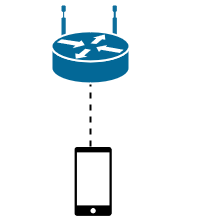
\includegraphics{exper1}
			\end{figure}
			\begin{itemize}
				\item Router TP-Link TD-W8970
				\begin{center}
					\begin{minipage}{\linewidth}
					Wersja bez przeszkody:\\\\
					\begin{tabular}{|c|c|c|}
						\hline 
						Pomiar & Siła sygnału (w dBm) & Obliczona odległość (w metrach) \\ 
						\hline 
						1 & -41 & 1,16 \\ 
						\hline 
						2 & -40 & 1,04 \\ 
						\hline 
						3 & -37 & 0.73 \\ 
						\hline 
						4 & -42 & 1.30 \\ 
						\hline 
						5 & -37 & 0,73 \\ 
						\hline 
					\end{tabular} 
				\end{minipage} 
				\end{center}
				\begin{center}
					\begin{minipage}{\linewidth}
						Wersja z przeszkodą:\\\\
					\begin{tabular}{|c|c|c|}
						\hline 
						Pomiar & Siła sygnału (w dBm) & Obliczona odległość (w metrach) \\ 
						\hline 
						1 & -38 & 0,82 \\ 
						\hline 
						2 & -39 & 0,92 \\ 
						\hline 
						3 & -42 & 1,30 \\ 
						\hline 
						4 & -46 & 2,07 \\ 
						\hline 
						7 & -43 & 1,46 \\ 
						\hline 
					\end{tabular}				
					\end{minipage} 
				\end{center}
			\item Router TP-Link TL-WA701ND
			\begin{center}
				\begin{minipage}{\linewidth}
					Wersja bez przeszkody:\\\\
					\begin{tabular}{|c|c|c|}
						\hline 
						Pomiar & Siła sygnału (w dBm) & Obliczona odległość (w metrach) \\ 
						\hline 
						1 & -44 & 0,98 \\ 
						\hline 
						2 & -44 & 0,98 \\ 
						\hline 
						3 & -45 & 1,10 \\ 
						\hline 
						4 & -47 & 1,38 \\ 
						\hline 
						5 & -45 & 1,10 \\ 
						\hline 
					\end{tabular} 
				\end{minipage} 
			\end{center}
			\begin{center}
				\begin{minipage}{\linewidth}
					Wersja z przeszkodą:\\\\
					\begin{tabular}{|c|c|c|}
						\hline 
						Pomiar & Siła sygnału (w dBm) & Obliczona odległość (w metrach) \\ 
						\hline 
						1 & -49 & 1,74 \\ 
						\hline 
						2 & -47 & 1,38 \\ 
						\hline 
						3 & -46 & 1,23 \\ 
						\hline 
						4 & -47 & 1,38 \\ 
						\hline 
						5 & -47 & 1,38 \\ 
						\hline 
					\end{tabular}//
				\end{minipage} 
			\end{center}
		\item Samsung Grand 2
		\begin{center}
			\begin{minipage}{\linewidth}
				Wersja bez przeszkody:\\\\
				\begin{tabular}{|c|c|c|}
					\hline 
					Pomiar & Siła sygnału (w dBm) & Obliczona odległość (w metrach) \\ 
					\hline 
					1 & -51 & 1,38 \\ 
					\hline 
					2 & -50 & 1,23 \\ 
					\hline 
					3 & -49 & 1,10 \\ 
					\hline 
					4 & -48 & 0,98 \\ 
					\hline 
					5 & -53 & 1,74 \\ 
					\hline 
				\end{tabular} 
			\end{minipage} 
		\end{center}
		\begin{center}
			\begin{minipage}{\linewidth}
				Wersja z przeszkodą:\\\\
				\begin{tabular}{|c|c|c|}
					\hline 
					Pomiar & Siła sygnału (w dBm) & Obliczona odległość (w metrach) \\ 
					\hline 
					1 & -50 & 1,23 \\ 
					\hline 
					2 & -54 & 1,95 \\ 
					\hline 
					3 & -53 & 1,74 \\ 
					\hline 
					4 & -55 & 2,19 \\ 
					\hline 
					5 & -55 & 2,19 \\ 
					\hline 
				\end{tabular}//
			\end{minipage} 
		\end{center}
		\end{itemize}
		
		\subsection{Pomiary zakłóceń}
		Eksperyment polegał na rozmieszczeniu trasmiterów na wierzchołkach trójkąta, w środku którego znajdował się odbiornik. Wszystkie urządzenia znajdowały się na tej samej wysokości. Mierzone były zmiany siły sygnału i obliczonej odległości w zależności od kąta położenia odbiornika w stosunku do trasmitera oraz ilości nakładających się na siebie sygnałów. Na początku, włączony był tylko transmiter o indeksie A. Odbiornik znajdował się w stosunku do transmitera pod kątem około 50 stopni. Następnie włączony został transmiter B. Na końcu do modelu został dodany trasmiter C.\\
		
		\begin{figure}				
			\centering
			\caption{Model systemu do pomiaru zakłóceń}
			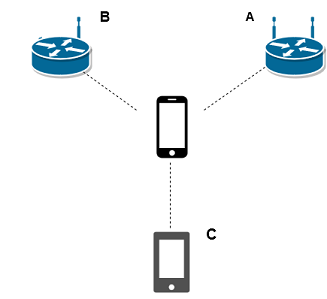
\includegraphics{inz2}
		\end{figure}
		Informacje o urządzeniach:
		\begin{itemize}
			\item Transmiter A - TP-Link TD-W8970, współrzędne (1.80, 0)
			\item Transmiter B - TP-Link TL-WA701ND, współrzędne (0, 0)
			\item Transmiter C - Samsung Grand 2, współrzędne (1.07, 1.8)
			\item Odbiornik - współrzędne (1.2, 0.45)
		\end{itemize}
		\begin{center}
			\begin{minipage}{\linewidth}
				Pomiar bez zakłóceń dla odległości 80cm przy kącie 50\textdegree :\\\\
				\begin{tabular}{|c|c|c|}
					\hline 
					Pomiar & Siła sygnału (w dBm) & Obliczona odległość (w metrach) \\ 
					\hline 
					1 & -41 & 1,16 \\ 
					\hline 
					2 & -43 & 1,46 \\ 
					\hline 
					3 & -41 & 1,16 \\ 
					\hline 
					4 & -42 & 1,30 \\ 
					\hline 
					5 & -43 & 1,46 \\ 
					\hline 
				\end{tabular}
			\end{minipage} 
		\end{center}
		\begin{center}
			\begin{minipage}{\linewidth}
				Pomiar z zakłóceniami z transmitera B dla odległości 80cm przy kącie 50\textdegree :\\\\
				\begin{tabular}{|c|c|c|}
					\hline 
					Pomiar & Siła sygnału (w dBm) & Obliczona odległość (w metrach) \\ 
					\hline 
					1 & -44 & 1,64 \\ 
					\hline 
					2 & -47 & 2,31 \\ 
					\hline 
					3 & -45 & 1,84 \\ 
					\hline 
					4 & -48 & 2,60 \\ 
					\hline 
					5 & -47 & 2,31 \\ 
					\hline 
				\end{tabular}
			\end{minipage} 
		\end{center}
		\begin{center}
			\begin{minipage}{\linewidth}
				Pomiar z zakłóceniami z obu transmiterów dla odległości 80cm przy kącie 50\textdegree :\\\\
				\begin{tabular}{|c|c|c|}
					\hline 
					Pomiar & Siła sygnału (w dBm) & Obliczona odległość (w metrach) \\ 
					\hline 
					1 & -48 & 2,60 \\ 
					\hline 
					2 & -47 & 2,31 \\ 
					\hline 
					3 & -44 & 1,64 \\ 
					\hline 
					4 & -48 & 2,60 \\ 
					\hline 
					5 & -46 & 2,06 \\ 
					\hline 
				\end{tabular}
			\end{minipage} 
		\end{center}
	\subsection{Wyznaczanie lokalizacji użytkownika}
	  Narazie mało do napisania. Z dwóch pomiarów dla modelu z góry, dostałem lokalizacje (-0,4; 1,2; -0,3) oraz (1,5; 1,67; -1,5).
\section{Model wyznaczania lokalizacji}
	Stworzyłem model algorytmu w MatLabie. Nie wyobrażam sobie modelu w trzech wymiarach i z kolorem (według mnie wynikiem będzie prostopadłościan o granatowym dominującym kolorze ścian) , dlatego stworzyłem model 2D, który jest tak naprawdę przekrojem modelu 3D (płaszczyzną XY).
	\begin{figure}	
		\centering			
		\caption{Model systemu z trzema routerami}
		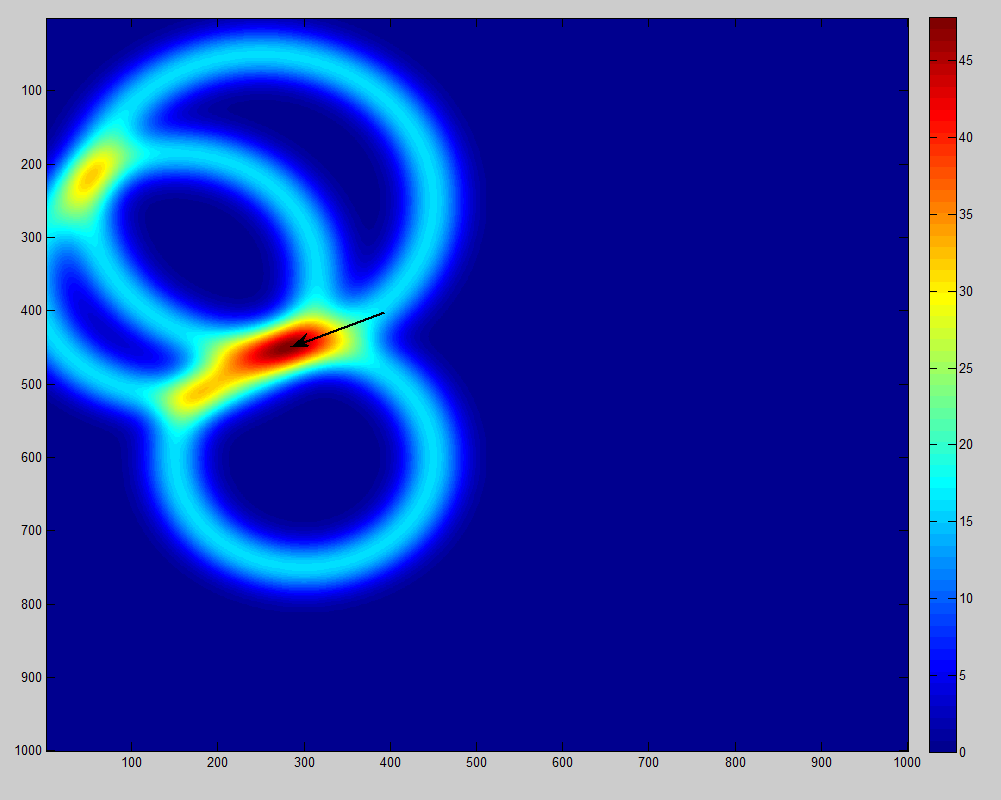
\includegraphics[width=\textwidth]{guasianRouter}
	\end{figure}
	Algorytm zmieniłem według zastrzeżeń Pana Doktora. Prostopadłościan, który zawiera w sobie "sfery" ruterów, dzielony jest na max 20 kawałków. Wyznacza się najlepszą pozycję, dla niej brane są sąsiadujące pozycję i uzyskany sześcian dzieli się na 9 kawałków i ponownie wyznacza najlepszą pozycję. Obliczenia kończą się, jak spełnione jest założenie: $szerKawalka \leqslant okreslonaDokladnosc$.	  
\end{document}